\subsection{Patrones de diseño}

\subsubsection{Composite}

\begin{figure}[H]
\centerline{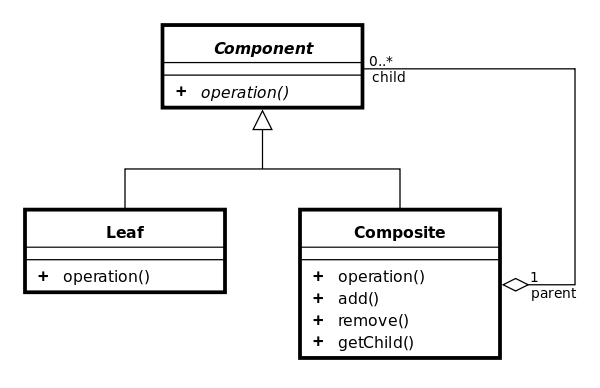
\includegraphics[width=7cm]{figuras/diseño/composite.png}}
\caption{Patrón de diseño Composite.}
\label{enlaceComposite}
\end{figure}

En esta aplicación se ha utilizado el patrón Composite \cite{composite}, el cual se refleja en la \hyperref[enlaceComposite]{Figura 3.6}, que se trata de un patrón estructural. Este permite la composición de objetos complejos a partir de otros más pequeños. 
\\

El ejemplo de este patrón de diseño es muy sencillo. Todas las páginas están formadas por distintos componentes: una cabecera, barra lateral, el propio cuerpo de la página, etc. En su conjunto, todos los componentes forman la página.


\subsubsection{Front Controller}

\begin{figure}[H]
\centerline{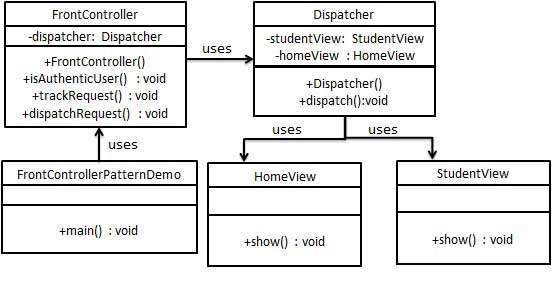
\includegraphics[width=7cm]{figuras/diseño/frontcontroller_pattern_uml_diagram.jpg}}
\caption{Patrón de diseño Front Controller.}
\label{enlaceFrontController}
\end{figure}

Otro patrón estructural utilizado es el Front Controller \cite{frontcontroller}, ilustrado en la \hyperref[enlaceFrontController]{Figura 3.7}. Este patrón es muy utilizado comunmente en las aplicaciones web, en las que una clase se encarga de recibir las entradas, llamando a los métodos necesarios para generar las salidas.
\\

En el caso de esta aplicación, la detección de este patrón es sencilla de ver. Se utilizan hasta cuatro controladores que llaman a sus respectivos servicios, donde se implementa la lógica de negocio. Estos controladores reciben las solicitudes HTTP desde el cliente, centralizando las llamadas, y solicitan las salidas a los diferentes servicios. Los controladores son: {\bf LocalController, XuntaController, AuthController} y {\bf UserController}.


\subsubsection{State}

En esta aplicación también se ha utilizado el patrón State \cite{state}, que se trata de un patrón de comportamiento. El objetivo es que el comportamiento de un objeto depende de su estado y cambia en tiempo de ejecución. 
\\

En React, la información se almacena localmente en estados ({\it state}). Cada vez que se actualiza un estado, varía el objeto que está referenciando dicho estado. En el caso de estar utilizando varios componentes para formar una página, cada vez que un componente se actualice, también lo hace la página que lo contiene.


\subsubsection{Hook}

El patrón Hook \cite{hooks} es también un patrón de comportamiento. Este es empleado para establecer un estado a los objetos de React sin ser necesario escribir una clase nueva.
\\

En toda la parte del cliente se han utilizado los hooks. Cada vez que se actualiza un estado, se está utilizando un hook nuevo. Además, en todas las llamadas a la API, se hace uso de la carpeta {\bf hooks}, la cual contiene hooks que actualizan el estado de elementos de la página, como puede ser una ley, los datos de un usuario, etc.